% ACS-style Methods draft: hybrid ML/MM training and MD (MMML).
% Compile:  tectonic -X compile main.tex
%           (or: make pdf)
% Target journal class: JCTC via achemso. Requires TeX Live / tectonic network fetch.
% Single-column review layout (ACS Paragon accepts author PDF); switch to
% layout=twocolumn for a production-like proof if desired.
\documentclass[journal=jctc,manuscript=article]{achemso}

%%%%%%%%%%%%%%%%%%%%%%%%
%%% Packages (minimal)
%%%%%%%%%%%%%%%%%%%%%%%%
\usepackage{amsmath,amssymb}
\usepackage{booktabs}
\usepackage{graphicx}
\usepackage{xcolor}
\usepackage{tikz}
\usetikzlibrary{
  arrows.meta,
  calc,
  fit,
  positioning,
  shapes.geometric,
  decorations.pathreplacing
}
\usepackage{siunitx}
\sisetup{per-mode=symbol}
\definecolor{MmBand}{RGB}{210,235,230}
\definecolor{MmLine}{RGB}{20,120,110}

%%%%%%%%%%%%%%%%%%%%%%%%
%%% Manuscript metadata
%%%%%%%%%%%%%%%%%%%%%%%%
\SectionNumbersOn
\renewcommand*\rmdefault{ptm}% Times-like body (ACS-friendly)

\author{Eric Boittier}
\affiliation{Department of Chemistry, University of Basel, Klingelbergstrasse 80, CH-4056 Basel, Switzerland}
\author{Markus Meuwly}
\affiliation{Department of Chemistry, University of Basel, Klingelbergstrasse 80, CH-4056 Basel, Switzerland}
\email{m.meuwly@unibas.ch}

\title{Hybrid Machine-Learning / Molecular-Mechanics Energy Functions for Condensed-Phase Simulations: Training and Molecular Dynamics}

\abbreviations{MD,ML,MM,COM,PME}
\keywords{machine learning, molecular mechanics, hybrid potentials, PhysNet, CHARMM, condensed phase}

\begin{document}

\begin{abstract}
We describe the hybrid machine-learning / molecular-mechanics (ML/MM) energy
function implemented in the MMML software stack and the associated training and
molecular-dynamics (MD) workflows. Intramolecular and short-range
intermolecular interactions are evaluated with a neural-network potential,
while intermolecular Lennard-Jones and Coulomb interactions are supplied by a
CHARMM/CGenFF-compatible classical term that is switched on as a function of
monomer center-of-mass separation. The same hybrid total energy is assembled
during supervised training (\texttt{physnet-train}) and during condensed-phase
MD (\texttt{md-system}), so that the learned model is trained on the Hamiltonian
later used for dynamics. Mechanical and electrostatic embeddings for the
classical Coulomb term are controlled by a charge-mode switch
(\texttt{fixed} versus \(\mathrm{Q}^{0}\)). Periodic long-range electrostatics
are provided by optional Ewald / particle-mesh Ewald solvers. The Methods
section below documents the energy decomposition, CLI entry points, default
handoff cutoffs, and campaign pipelines used for liquid dichloromethane,
acetone, and methane.
\end{abstract}

\tableofcontents
\clearpage

%%%%%%%%%%%%%%%%%%%%%%%%%%%%%%%%%%%%%%%%%%%%%%%%%%%%%%%%%%%%%%%%%%%%%%%%%%%%%%%
\section{Introduction}
%%%%%%%%%%%%%%%%%%%%%%%%%%%%%%%%%%%%%%%%%%%%%%%%%%%%%%%%%%%%%%%%%%%%%%%%%%%%%%%

Machine-learned (ML) potentials offer near-quantum accuracy for local chemical
environments, but long-range electrostatics and large condensed-phase systems
remain expensive when treated entirely by neural networks. Classical molecular
mechanics (MM) force fields such as CHARMM/CGenFF\cite{Vanommeslaeghe2010,Brooks2009CHARMM}
remain efficient for intermolecular interactions at longer range. Hybrid ML/MM
energy functions combine the two: ML for intramolecular and short-range
many-body interactions, and MM for the intermolecular tail and optional
long-range Coulomb solvers.\cite{Unke2019PhysNet,MMML2026}

A practical hybrid scheme must expose a \emph{single} total energy both when
fitting parameters and when integrating equations of motion. The MMML package
implements that requirement through a shared hybrid forward pass used by the
\texttt{physnet-train} and \texttt{md-system} commands. The remainder of this
article details the hybrid energy (Section~\ref{sec:energy}), training
(Section~\ref{sec:train}), MD campaigns (Section~\ref{sec:md}), charge
embeddings (Section~\ref{sec:charges}), and software reproducibility
(Section~\ref{sec:software}).

%%%%%%%%%%%%%%%%%%%%%%%%%%%%%%%%%%%%%%%%%%%%%%%%%%%%%%%%%%%%%%%%%%%%%%%%%%%%%%%
\section{Hybrid ML/MM Energy Function}
\label{sec:energy}
%%%%%%%%%%%%%%%%%%%%%%%%%%%%%%%%%%%%%%%%%%%%%%%%%%%%%%%%%%%%%%%%%%%%%%%%%%%%%%%

\subsection{Monomer Partition and Center-of-Mass Switching}

Interactions are partitioned by \emph{monomer} (typically one solvent residue).
Let \(r_{IJ}\) denote the center-of-mass (COM) distance between monomers \(I\)
and \(J\). The hybrid potential takes the form
\begin{multline}
\label{eq:hybrid-E}
E = \sum_I E_I^{\mathrm{ML}}
  + \sum_{I<J}\bigl[
        s_{\mathrm{ML}}(r_{IJ})\,E_{IJ}^{\mathrm{ML}}
      + s_{\mathrm{MM}}(r_{IJ})\,E_{IJ}^{\mathrm{MM}}
    \bigr] \\
  + E^{\mathrm{LR}} + E^{\mathrm{wall/restr}}.
\end{multline}
where \(E_I^{\mathrm{ML}}\) is the intramolecular ML energy of monomer \(I\),
\(E_{IJ}^{\mathrm{ML}}\) is the ML two-body (dimer) correction, and
\(E_{IJ}^{\mathrm{MM}}\) collects switched intermolecular Lennard-Jones and
Coulomb contributions evaluated with CGenFF-compatible parameters. Optional
long-range Coulomb beyond the real-space switch enters as \(E^{\mathrm{LR}}\)
(Ewald\cite{Ewald1921}, particle-mesh Ewald, or related solvers). A short-range
steric wall and restraints may contribute \(E^{\mathrm{wall/restr}}\).

For an isolated dimer \(AB\), Equation~\ref{eq:hybrid-E} is equivalent to the
training assembly
\begin{equation}
\label{eq:dimer-train}
E = (1-s)\,(E_A+E_B) + s\,E_{AB} + E_{\mathrm{MM}},
\end{equation}
with \(s=s_{\mathrm{ML}}(r_{\mathrm{COM}})\),
\(\Delta E_{\mathrm{ML}}=E_{AB}-E_A-E_B\), and
\(E=E_A+E_B+s\,\Delta E_{\mathrm{ML}}+E_{\mathrm{MM}}\).
The taper multiplies only the \emph{dimer interaction}; monomer intramolecular
energies remain fully on at all separations. Forces include the product-rule
term arising from \(\partial s/\partial\mathbf{R}\).

\subsection{Default Handoff Window}

With complementary handoff, \(s_{\mathrm{ML}}+s_{\mathrm{MM}}=1\) inside the
ML\(\leftrightarrow\)MM transition. Production defaults used throughout training
and MD YAML are listed in Table~\ref{tab:cutoffs} and illustrated in
Figure~\ref{fig:handoff}.

\begin{table}[h]
\caption{Default COM handoff parameters shared by \texttt{physnet-train} and
\texttt{md-system}.}
\label{tab:cutoffs}
\begin{tabular}{llc}
\toprule
Parameter & Symbol / role & Default \\
\midrule
\texttt{mm\_switch\_on} & end of ML\(\to\)MM handoff & \SI{8.0}{\angstrom} \\
\texttt{ml\_switch\_width} & ML taper width & \SI{1.5}{\angstrom} \\
\texttt{mm\_switch\_width} & MM outer tail & \SI{5.0}{\angstrom} \\
\bottomrule
\end{tabular}
\end{table}

\begin{figure}[t]
\centering
\resizebox{\textwidth}{!}{%
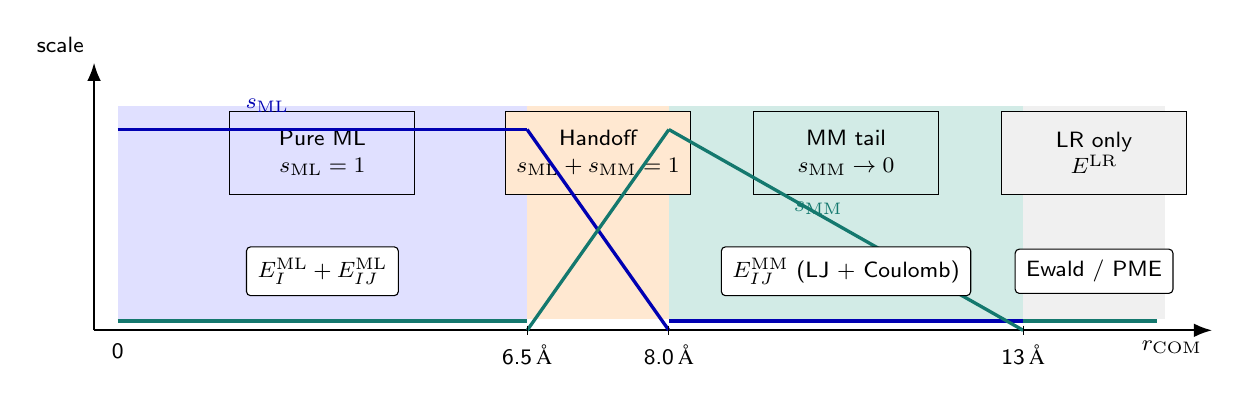
\begin{tikzpicture}[
  font=\footnotesize\sffamily,
  >=Latex,
  box/.style={draw, rounded corners=1.5pt, align=center, inner sep=4pt},
  band/.style={draw, minimum height=1.05cm, minimum width=2.35cm, align=center},
]
  % axis
  \draw[->, thick] (0,0) -- (14.2,0) node[below left] {$r_{\mathrm{COM}}$};
  \draw[->, thick] (0,0) -- (0,3.4) node[above left] {scale};

  % region bands
  \fill[blue!12] (0.3,0.15) rectangle (5.5,2.85);
  \fill[orange!18] (5.5,0.15) rectangle (7.3,2.85);
  \fill[MmBand] (7.3,0.15) rectangle (11.8,2.85);
  \fill[gray!12] (11.8,0.15) rectangle (13.6,2.85);

  \node[band, fill=blue!12] at (2.9,2.25) {Pure ML\\$s_{\mathrm{ML}}=1$};
  \node[band, fill=orange!18] at (6.4,2.25) {Handoff\\$s_{\mathrm{ML}}+s_{\mathrm{MM}}=1$};
  \node[band, fill=MmBand] at (9.55,2.25) {MM tail\\$s_{\mathrm{MM}}\to 0$};
  \node[band, fill=gray!12] at (12.7,2.25) {LR only\\$E^{\mathrm{LR}}$};

  % switch curves (schematic)
  \draw[blue!70!black, very thick, domain=0.3:5.5, samples=40] plot (\x,{2.55});
  \draw[blue!70!black, very thick, domain=5.5:7.3, samples=50]
    plot (\x,{2.55*(7.3-\x)/(7.3-5.5)});
  \draw[blue!70!black, very thick, domain=7.3:13.5, samples=20] plot (\x,{0.12});
  \node[blue!70!black] at (2.2,2.85) {$s_{\mathrm{ML}}$};

  \draw[MmLine, very thick, domain=0.3:5.5, samples=20] plot (\x,{0.12});
  \draw[MmLine, very thick, domain=5.5:7.3, samples=50]
    plot (\x,{2.55*(\x-5.5)/(7.3-5.5)});
  \draw[MmLine, very thick, domain=7.3:11.8, samples=50]
    plot (\x,{2.55*(11.8-\x)/(11.8-7.3)});
  \draw[MmLine, very thick, domain=11.8:13.5, samples=20] plot (\x,{0.12});
  \node[MmLine] at (9.2,1.55) {$s_{\mathrm{MM}}$};

  % ticks
  \foreach \x/\lab in {5.5/6.5, 7.3/8.0, 11.8/13} {
    \draw (\x,0.06) -- (\x,-0.06) node[below] {\lab\,\si{\angstrom}};
  }
  \node[below] at (0.3,-0.05) {0};

  % ownership callouts
  \node[box, fill=white] at (2.9,0.75) {$E_I^{\mathrm{ML}}+E_{IJ}^{\mathrm{ML}}$};
  \node[box, fill=white] at (9.55,0.75) {$E_{IJ}^{\mathrm{MM}}$ (LJ + Coulomb)};
  \node[box, fill=white] at (12.7,0.75) {Ewald / PME};
\end{tikzpicture}%
}
\caption{Schematic COM handoff for the hybrid energy in Equation~\ref{eq:hybrid-E}.
Below \(\approx\SI{6.5}{\angstrom}\) the intermolecular ML dimer term is fully
on; between \SI{6.5}{\angstrom} and \SI{8.0}{\angstrom} ML and MM scales are
complementary; the switched MM pair term decays by \SI{13}{\angstrom}. Beyond
the MM cutoff, only optional long-range Coulomb (\(E^{\mathrm{LR}}\)) remains.}
\label{fig:handoff}
\end{figure}

\subsection{Ownership of Terms}

Table~\ref{tab:ownership} summarizes which component owns each contribution.
Nuclear repulsion inside the neural model (optional Ziegler--Biersack--Littmark,
ZBL) is distinct from the classical short-range wall used as a safety term
outside the training domain.

\begin{table}[h]
\caption{Term ownership in the hybrid Hamiltonian.}
\label{tab:ownership}
\begin{tabular}{llp{4.6cm}}
\toprule
Term & Owner & Notes \\
\midrule
\(E_I^{\mathrm{ML}}\) & PhysNet / Spooky & Always on \\
\(E_{IJ}^{\mathrm{ML}}\) & PhysNet / Spooky & COM-gated by \(s_{\mathrm{ML}}\) \\
LJ + Coulomb pairs & CGenFF MM & Scaled by \(s_{\mathrm{MM}}\); \(q\) from charge mode \\
Optional LJ scales & Trainable \(s^\sigma,s^\varepsilon\) & Sidecar \texttt{hybrid\_mm.json} \\
\(E^{\mathrm{LR}}\) & Ewald / PME / \ldots & \texttt{lr\_solver} \\
Bonded CHARMM & Topology (Mode~B) & Or jax-mm-spoof bonded clone \\
\bottomrule
\end{tabular}
\end{table}

%%%%%%%%%%%%%%%%%%%%%%%%%%%%%%%%%%%%%%%%%%%%%%%%%%%%%%%%%%%%%%%%%%%%%%%%%%%%%%%
\section{Hybrid Training}
\label{sec:train}
%%%%%%%%%%%%%%%%%%%%%%%%%%%%%%%%%%%%%%%%%%%%%%%%%%%%%%%%%%%%%%%%%%%%%%%%%%%%%%%

\subsection{CLI Entry Point and Dataset}

Hybrid models are trained with
\begin{center}
\texttt{mmml physnet-train --hybrid-mm [--config train.yaml]}
\end{center}
The CLI is implemented in \texttt{mmml/cli/make/make\_training.py}. Training
targets the \emph{hybrid} total of Equation~\ref{eq:dimer-train}, not the bare
neural energy, so that the checkpoint used later in MD matches the dynamics
Hamiltonian.

Datasets are covalent \emph{dimers}: each frame contains exactly two monomers.
In addition to standard QM labels (\(R\), \(Z\), \(E\), \(\mathbf{F}\), optional
dipole/charges), NPZ files must provide CGenFF fields
(\texttt{cgenff\_type\_idx}, \texttt{mol\_id}, \texttt{cgenff\_charge},
\texttt{cgenff\_master\_sigmas}/\texttt{epsilons}). These fields are prepared by
\texttt{mmml prepare-mm-dataset} after electronic-structure evaluation of
normal-mode samples.

\subsection{Loss and Key Flags}

The supervised objective is a weighted sum of squared residuals on hybrid
energies and forces (and optional dipole / charge heads),
\begin{equation}
\label{eq:loss}
\mathcal{L}
  = w_E\|E-E^{\mathrm{ref}}\|^2
  + w_F\|\mathbf{F}-\mathbf{F}^{\mathrm{ref}}\|^2
  + w_D\|\boldsymbol{\mu}-\boldsymbol{\mu}^{\mathrm{ref}}\|^2
  + w_q\|q-q^{\mathrm{ref}}\|^2.
\end{equation}
Representative weights used in the bundled fixed-charge template are
\(w_E=1\), \(w_F=52.91\), \(w_D=27.21\), and \(w_q=14.39\). Validation scores
the same hybrid total.

Essential flags (YAML or CLI) are summarized below. The PhysNet radial cutoff
must be at least \texttt{mm\_switch\_on}. Portable JSON checkpoints (and
optional \texttt{hybrid\_mm.json} LJ-scale sidecars) are written for MD
deployment. Figure~\ref{fig:train} summarizes the pipeline.
\begin{itemize}
\item \texttt{--hybrid-mm} --- enable hybrid total of Equation~\ref{eq:dimer-train}
\item \texttt{--mm-charge-mode} \(\{\texttt{fixed},\texttt{q0},\texttt{latent},\ldots\}\)
\item \texttt{--charges} / \texttt{--no-charges} --- neural charge head
\item \texttt{--ml-switch-width}, \texttt{--mm-switch-on}, \texttt{--mm-switch-width}
  (Table~\ref{tab:cutoffs})
\item \texttt{--lr-solver} \(\{\texttt{mic},\texttt{ewald},\texttt{nvalchemiops\_pme}\}\)
\item \texttt{--learn-mm-lj-scales} --- optional trainable LJ scales
\end{itemize}

\begin{figure}[t]
\centering
\resizebox{\textwidth}{!}{%
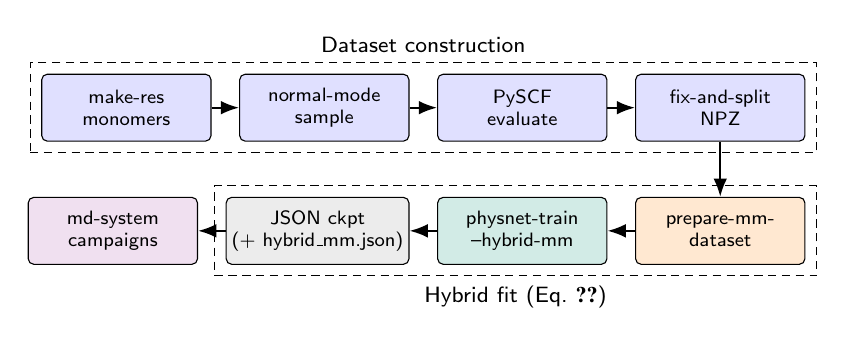
\begin{tikzpicture}[
  font=\scriptsize\sffamily,
  >=Latex,
  node distance=0.45cm and 0.35cm,
  step/.style={draw, rounded corners=2pt, align=center, fill=#1,
               minimum width=2.15cm, minimum height=0.85cm, inner sep=2pt},
  step/.default=black!6,
  arr/.style={->, thick},
]
  \node[step=blue!12] (res) {make-res\\monomers};
  \node[step=blue!12, right=of res] (nms) {normal-mode\\sample};
  \node[step=blue!12, right=of nms] (qm) {PySCF\\evaluate};
  \node[step=blue!12, right=of qm] (split) {fix-and-split\\NPZ};
  \node[step=orange!18, below=0.7cm of split] (prep) {prepare-mm-\\dataset};
  \node[step=MmBand, left=of prep] (train) {physnet-train\\--hybrid-mm};
  \node[step=gray!15, left=of train] (ckpt) {JSON ckpt\\(+ hybrid\_mm.json)};
  \node[step=violet!12, left=of ckpt] (md) {md-system\\campaigns};

  \draw[arr] (res) -- (nms);
  \draw[arr] (nms) -- (qm);
  \draw[arr] (qm) -- (split);
  \draw[arr] (split) -- (prep);
  \draw[arr] (prep) -- (train);
  \draw[arr] (train) -- (ckpt);
  \draw[arr] (ckpt) -- (md);

  \node[draw, densely dashed, fit=(res)(nms)(qm)(split),
        inner sep=4pt, label=above:{\footnotesize Dataset construction}] {};
  \node[draw, densely dashed, fit=(prep)(train)(ckpt),
        inner sep=4pt, label=below:{\footnotesize Hybrid fit (Eq.~\ref{eq:dimer-train})}] {};
\end{tikzpicture}%
}
\caption{Hybrid training pipeline. Quantum labels on dimer geometries are
augmented with CGenFF arrays, then \texttt{physnet-train --hybrid-mm} fits the
hybrid total of Equation~\ref{eq:dimer-train}. The resulting portable JSON
checkpoint is consumed unchanged by \texttt{md-system}.}
\label{fig:train}
\end{figure}

%%%%%%%%%%%%%%%%%%%%%%%%%%%%%%%%%%%%%%%%%%%%%%%%%%%%%%%%%%%%%%%%%%%%%%%%%%%%%%%
\section{Condensed-Phase Molecular Dynamics}
\label{sec:md}
%%%%%%%%%%%%%%%%%%%%%%%%%%%%%%%%%%%%%%%%%%%%%%%%%%%%%%%%%%%%%%%%%%%%%%%%%%%%%%%

\subsection{CLI Entry Point and Campaign YAML}

Dynamics are launched with
\begin{center}
\texttt{mmml md-system --config campaign.yaml --run-all [--resume]}
\end{center}
(\texttt{mmml/cli/run/md\_system.py}). A campaign file supplies global
\texttt{defaults} (composition, box, checkpoint, cutoffs, \texttt{lr\_solver},
\texttt{mm\_charge\_mode}, backend options) and an ordered list of
\texttt{runs}/\texttt{jobs}. Dependencies are resolved automatically; each leg
writes a handoff state (\texttt{handoff/state.npz}) consumed by the next stage.

Supported backends are \texttt{pycharmm} (CHARMM integrator with MLpot USER
callback),\cite{Brooks2009CHARMM} \texttt{jaxmd} (pure-JAX evaluation with a
jax-md integrator),\cite{Schoenholz2019JaxMD} and \texttt{ase} for reference
smokes. Ensembles include \texttt{pbc\_nvt}, \texttt{pbc\_npt}, and
\texttt{pbc\_nve}.

\subsection{Two Drivers, One Hamiltonian}

\begin{itemize}
\item \textbf{Mode A (jax-md).} CHARMM is used only to build the topology;
  every energy term is evaluated in a jitted hybrid energy function.
\item \textbf{Mode B (PyCHARMM).} CHARMM advances the trajectory; the hybrid ML
  contribution enters each step through the MLpot callback while classical
  bonded / nonbonded bookkeeping follows the PSF.
\end{itemize}
Both drivers evaluate Equation~\ref{eq:hybrid-E} with the same handoff
parameters and charge mode.

\subsection{Box Preparation and Dynamics Stages}

Dense liquids follow a two-phase protocol (Figure~\ref{fig:md}):
\begin{enumerate}
\item \textbf{Phase A (MM certify).} Packmol placement, optional Monte Carlo
  density moves, and classical minimization / short dynamics until
  inter-monomer contact criteria pass.
\item \textbf{Phase B (hybrid MD).} Register the ML potential (or a jax-mm-spoof
  bonded clone for infrastructure tests), minimize under the hybrid energy,
  then heat \(\to\) equilibrate \(\to\) produce.
\end{enumerate}
Optional CHARMM MM pretreat (\texttt{pretreat\_on\_pycharmm}) inserts short
classical heat/equilibration before MLpot registration on dense boxes.

\begin{figure}[t]
\centering
\resizebox{\textwidth}{!}{%
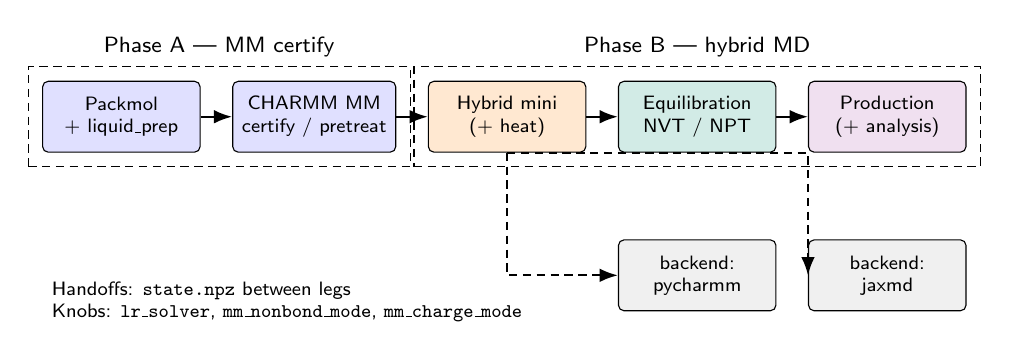
\begin{tikzpicture}[
  font=\scriptsize\sffamily,
  >=Latex,
  node distance=0.55cm and 0.4cm,
  box/.style={draw, rounded corners=2pt, align=center, fill=#1,
              minimum width=2.0cm, minimum height=0.9cm},
  box/.default=black!6,
  arr/.style={->, thick},
]
  \node[box=blue!12] (pack) {Packmol\\+ liquid\_prep};
  \node[box=blue!12, right=of pack] (mm) {CHARMM MM\\certify / pretreat};
  \node[box=orange!18, right=of mm] (mini) {Hybrid mini\\(+ heat)};
  \node[box=MmBand, right=of mini] (equi) {Equilibration\\NVT / NPT};
  \node[box=violet!12, right=of equi] (prod) {Production\\(+ analysis)};

  \draw[arr] (pack) -- (mm);
  \draw[arr] (mm) -- (mini);
  \draw[arr] (mini) -- (equi);
  \draw[arr] (equi) -- (prod);

  % fork backends
  \node[box=gray!12, below=1.1cm of equi] (py) {backend:\\pycharmm};
  \node[box=gray!12, below=1.1cm of prod] (jx) {backend:\\jaxmd};
  \draw[arr, densely dashed] (mini.south) |- (py.west);
  \draw[arr, densely dashed] (mini.south) -| (jx.west);

  \node[draw, densely dashed, fit=(pack)(mm), inner sep=5pt,
        label=above:{\footnotesize Phase A --- MM certify}] {};
  \node[draw, densely dashed, fit=(mini)(equi)(prod), inner sep=5pt,
        label=above:{\footnotesize Phase B --- hybrid MD}] {};

  \node[align=left, anchor=west] at ($(pack.west)+(0,-2.35)$) {
    Handoffs: \texttt{state.npz} between legs\\
    Knobs: \texttt{lr\_solver}, \texttt{mm\_nonbond\_mode}, \texttt{mm\_charge\_mode}
  };
\end{tikzpicture}%
}
\caption{Condensed-phase campaign pipeline driven by \texttt{md-system --run-all}.
Phase~A builds and certifies a classical liquid box; Phase~B registers the hybrid
potential and runs mini/heat/equilibration/production on either the PyCHARMM or
jax-md backend. Long-range Coulomb and charge embedding are selected in campaign
defaults and applied identically on both backends.}
\label{fig:md}
\end{figure}

\subsection{Paper Workflows}

Two Snakemake workflows instantiate the campaign pattern for the manuscript:
\begin{itemize}
\item \texttt{workflows/pbc\_liquid\_density\_dyn/} --- dichloromethane and acetone
  liquids under NPT/NVT with density acceptance metrics;
\item \texttt{workflows/pbc\_methane\_ewald/} --- methane at fixed liquid density
  with \texttt{lr\_solver: ewald} and \texttt{mm\_nonbond\_mode: periodic\_external},
  sweeping temperature, checkpoint, backend, and embedding
  (mechanical / electrostatic).
\end{itemize}

%%%%%%%%%%%%%%%%%%%%%%%%%%%%%%%%%%%%%%%%%%%%%%%%%%%%%%%%%%%%%%%%%%%%%%%%%%%%%%%
\section{Mechanical and Electrostatic Embeddings}
\label{sec:charges}
%%%%%%%%%%%%%%%%%%%%%%%%%%%%%%%%%%%%%%%%%%%%%%%%%%%%%%%%%%%%%%%%%%%%%%%%%%%%%%%

The classical Coulomb term inside \(E_{\mathrm{MM}}\) obtains its per-atom
charges from \texttt{mm\_charge\_mode}. This choice is orthogonal to whether the
neural model predicts charges for use \emph{inside} \(E^{\mathrm{ML}}\).

\begin{description}
\item[Mechanical embedding (\texttt{fixed}).]
  \(q_{\mathrm{MM}}=q_{\mathrm{CGenFF}}\). Default for charge-less PhysNet
  checkpoints (e.g., DES dimers) and for LJ-fitting stages.
\item[Electrostatic embedding (\texttt{q0} / \(\mathrm{Q}^{0}\)).]
  \(q_{\mathrm{MM}}=\mathrm{neutralize}(Q^{0})\), where \(Q^{0}\) denotes
  unperturbed monomer charge-head evaluations. Requires a charge-capable
  checkpoint (\texttt{charges: true}). Suitable for liquids.
\item[Dimer-only modes (\texttt{latent}/\(\mathrm{Q}^{1}\), \texttt{fixed\_plus\_latent}).]
  Partner-perturbed charges from the \(AB\) forward; undefined for \(N>2\)
  monomers and therefore not used in liquid production matrices.
\end{description}

Figure~\ref{fig:embed} contrasts the two liquid-capable embeddings used in the
methane Ewald smoke matrix. Campaign tags encode the choice as \texttt{\_mech\_}
or \texttt{\_es\_}.

\begin{figure}[t]
\centering
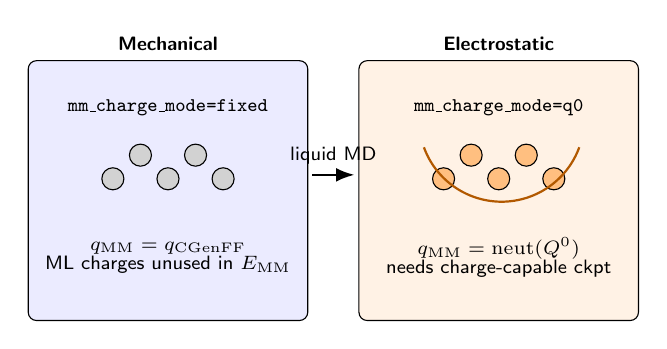
\begin{tikzpicture}[
  font=\scriptsize\sffamily,
  >=Latex,
  pane/.style={draw, rounded corners=3pt, fill=#1, minimum width=3.55cm,
               minimum height=3.3cm, align=center},
  atom/.style={circle, draw, inner sep=0pt, minimum size=0.28cm},
  arr/.style={->, thick},
]
  % Mechanical
  \node[pane=blue!8] (M) at (0,0) {};
  \node[above] at (M.north) {\textbf{Mechanical}};
  \node at ($(M.center)+(0,1.05)$) {\texttt{mm\_charge\_mode=fixed}};
  \foreach \x/\y in {-0.7/0.15, -0.35/0.45, 0.0/0.15, 0.35/0.45, 0.7/0.15} {
    \node[atom, fill=gray!35] at ($(M.center)+(\x,\y)$) {};
  }
  \node[align=center] at ($(M.center)+(0,-0.85)$)
    {$q_{\mathrm{MM}}=q_{\mathrm{CGenFF}}$\\[-1pt]
     ML charges unused in \(E_{\mathrm{MM}}\)};

  % Electrostatic
  \node[pane=orange!10] (E) at (4.2,0) {};
  \node[above] at (E.north) {\textbf{Electrostatic}};
  \node at ($(E.center)+(0,1.05)$) {\texttt{mm\_charge\_mode=q0}};
  \foreach \x/\y in {-0.7/0.15, -0.35/0.45, 0.0/0.15, 0.35/0.45, 0.7/0.15} {
    \node[atom, fill=orange!50] at ($(E.center)+(\x,\y)$) {};
  }
  \draw[orange!70!black, thick] ($(E.center)+(-0.95,0.55)$) arc (200:340:1.05);
  \node[align=center] at ($(E.center)+(0,-0.85)$)
    {$q_{\mathrm{MM}}=\mathrm{neut}(Q^{0})$\\[-1pt]
     needs charge-capable ckpt};

  \draw[arr] ($(M.east)+(0.05,0.2)$) -- ($(E.west)+(-0.05,0.2)$)
    node[midway, above] {liquid MD};
\end{tikzpicture}
\caption{Liquid-capable embeddings for hybrid MM Coulomb. Mechanical embedding
keeps fixed CGenFF charges in \(E_{\mathrm{MM}}\). Electrostatic embedding
(\(\mathrm{Q}^{0}\)) rebuilds neutralized monomer ML charges each evaluation.
Dimer-only \(\mathrm{Q}^{1}\) modes are omitted from condensed-phase matrices.}
\label{fig:embed}
\end{figure}

%%%%%%%%%%%%%%%%%%%%%%%%%%%%%%%%%%%%%%%%%%%%%%%%%%%%%%%%%%%%%%%%%%%%%%%%%%%%%%%
\section{Software and Reproducibility}
\label{sec:software}
%%%%%%%%%%%%%%%%%%%%%%%%%%%%%%%%%%%%%%%%%%%%%%%%%%%%%%%%%%%%%%%%%%%%%%%%%%%%%%%

Table~\ref{tab:soft} lists the principal components. Manuscript figures and
tables are regenerable from versioned Snakemake workflows under
\texttt{workflows/}; each Results entry should cite the workflow directory,
config file, artifact path, and git commit. Engineering smoke matrices
(including DES / So3LR methane Ewald cells with mechanical and electrostatic
embeddings) are recorded in the accompanying Results draft and are not
themselves production property claims.

\begin{table}[h]
\caption{Software stack for hybrid training and MD.}
\label{tab:soft}
\begin{tabular}{lp{5.2cm}}
\toprule
Component & Role \\
\midrule
MMML (\texttt{mmml})\cite{MMML2026} & CLI, hybrid calculator, workflows \\
\texttt{physnet-train} & Hybrid supervised training \\
\texttt{md-system} & Campaign MD (ASE / jax-md / PyCHARMM) \\
JAX / jax-md\cite{Schoenholz2019JaxMD} & Differentiable hybrid energy; jaxmd backend \\
PyCHARMM / CHARMM\cite{Brooks2009CHARMM} & Topology, classical MM, pycharmm backend \\
Snakemake (+ Slurm) & Parameter sweeps and cluster submission \\
\bottomrule
\end{tabular}
\end{table}

%%%%%%%%%%%%%%%%%%%%%%%%%%%%%%%%%%%%%%%%%%%%%%%%%%%%%%%%%%%%%%%%%%%%%%%%%%%%%%%
\section{Conclusions}
%%%%%%%%%%%%%%%%%%%%%%%%%%%%%%%%%%%%%%%%%%%%%%%%%%%%%%%%%%%%%%%%%%%%%%%%%%%%%%%

The hybrid ML/MM formulation in Equation~\ref{eq:hybrid-E}, the training
assembly in Equation~\ref{eq:dimer-train}, and the \texttt{md-system} campaign
protocol provide a closed loop from dimer QM data to condensed-phase dynamics.
Mechanical (\texttt{fixed}) and electrostatic (\(\mathrm{Q}^{0}\)) embeddings
select how classical Coulomb charges are obtained without changing the ML/MM
ownership of bonded and short-range many-body terms. Shared handoff defaults
and portable JSON checkpoints keep training and MD numerically aligned across
the jax-md and PyCHARMM drivers.

%%%%%%%%%%%%%%%%%%%%%%%%%%%%%%%%%%%%%%%%%%%%%%%%%%%%%%%%%%%%%%%%%%%%%%%%%%%%%%%
\begin{acknowledgement}
We thank members of the Meuwly group for discussions on hybrid ML/MM workflows.
Computational resources at the University of Basel are gratefully acknowledged.
\end{acknowledgement}

%%%%%%%%%%%%%%%%%%%%%%%%%%%%%%%%%%%%%%%%%%%%%%%%%%%%%%%%%%%%%%%%%%%%%%%%%%%%%%%
\begin{suppinfo}
Extended CLI flag tables, YAML templates under
\texttt{examples/hybrid\_mm\_charges/}, and workflow provenance maps are
available in the MMML documentation tree
\texttt{docs/manuscripts/condensed-phase-hybrid-mlmm/}.
\end{suppinfo}

\bibliography{refs}

\end{document}
